% on Windows 10 bash(ubuntu 14.04), you need to:
% apt install texlive-latex-extra texlive-latex-recommended latex-xcolor latexmk make python-pygments
\documentclass[twocolumn]{article}

% T1 fonts not available on the default windows latex
%\usepackage[T1]{fontenc}
%\usepackage{lmodern}

\usepackage[pdftex]{graphicx}
\usepackage{xcolor}
\setlength{\parindent}{0cm}
\setlength{\columnsep}{25pt}
\usepackage{minted}
\newminted{cpp}{mathescape,linenos,frame=single,numbersep=0.5mm}
\definecolor{almostnogray}{rgb}{0.92,0.92,0.92}


\sloppy

% Your name
\author{Clemens Ruck \& Alex Egger\\ Technische Universit\"at M\"unchen}

\title{Proseminar ``The Rust Programming Language'' \\
       Summer Term 2017 \\
       {\bf Garbage Collection and Reference Counting}
}

% Date of your talk
\date{9.6.2017}

\begin{document}

\maketitle

\begin{abstract}
The main focus of this paper is to give a broad overview
of existing memory management techniques, and more specifically
to compare them to the approach chosen by the Rust language.
Further it will cover the subject of how to use memory effectively in the Rust language.
\end{abstract}

% \section defines numbered parts of the paper with titles
% there also are \subsection and \subsubsection
\section{Introduction}

% Use labels to be able to refer to this position from somewhere else
\label{introduction}


The introduction of a scientific work usually consists of the following
parts:
\begin{itemize}
	\item motivation,
	\item issues or drawbacks with existing solutions of a problem at hand,
	\item overview of new contribution and rest of the paper.
\end{itemize}
In the motivation you should explain why a given topic is interesting
at all, and also, why solutions are important from a scientific point
of view. There already may be a lot of existing solutions. Thus, it
is important for the reader to understand the issues with these solutions,
and why they are not enough for e.g. a specific scenario. Often, concrete
examples are quite useful in providing a motivation, as well as providing
a running example, that can be picked up later on in the main part.
\begin{figure}
\begin{cppcode}
#include <iostream>
void main(void){
  std::cout << "simple code example";
}
\end{cppcode}

\vspace{-2em}
\caption{A very simple C++ code fragment}
\label{introexample}
\end{figure}
After the motivational example, you should explain the basic idea of your new
contribution to solve the problem at hand, and give a short overview
(only a slight hint) of how this works.

\subsection*{Related Work}

Here, you elaborate on how this approach differs from other existing solutions -- if not in general, then illustrate the scenario, in which the approach is beneficial. This subsection also offers room for introducing related or alternative approaches to this approach, and establishes a kind of state of the art. This might even incorporate solution approaches in other fields, if the setting is comparable to this thesis. Translated to topics in programming languages, this would mean e.g. similar solutions in other programming languages. Ultimately, however, this should culminate in explicitely formulating the \emph{thesis statement} \cite{thesis-statement}:
\begin{itemize}
\item what is the unique core contribution of this specific approach
\item in not more than 3 itemss
\item this should be thought of the basic information, that the reader
  should take away from your paper
\end{itemize}
This concept of unique core contributions is in seminar papers, what in
research papers is usually the \emph{Research Question} \cite{constructing-research-questions}. As the seminar paper is usually meant to be a piece of
work, that teaches students to write academic papers, the usual guides
for general scientific writing like the work of Turabian \cite{manual-for-writers} or the more computer science centric approach of Zobel
\cite{writing-for-computer-science} can also be applied to seminar papers.


Finally, a short overview to the structure of the rest of the work
should be provided, which may indicate the most important points.
As any idea or solution proposed must be shown to be valid and useful, every scientific paper
must have some evaluation and/or discussion. It may to useful to select
important results, and mention them already as last part of the
introduction, as motivation for the reader to read on. In summary,
a good introduction creates interest for the topic and
proposed new contributions that the reader cannot wait to read on.

% free floating figure using width of one column.
\begin{figure}
\centerline{

\includegraphics[width=0.9\columnwidth,interpolate]{Figures/TUM-Logo-102.png}
}
\caption{The caption explaining what can be seen in the image/figure.
Readers often read captions first if they do not have much time. Thus,
it is important to find a good short explanation.}
% A label to allow refering to this figure in the text.
\label{TUM}
\end{figure}

% free floating figure using width of full page, to be put on [t]op.
\begin{figure*}[t]
\centerline{
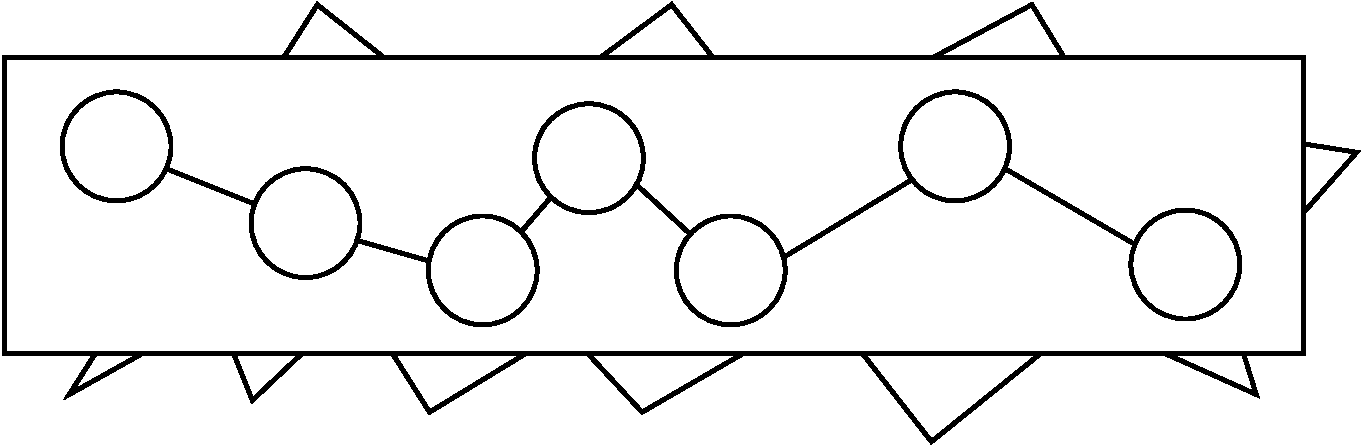
\includegraphics[width=0.9\textwidth]{Figures/test.pdf}
}
\caption{A nice caption. The larger width allows for more text without
taking too much space.}
\label{Fig2}
\end{figure*}

\section{Paper organization}
The main part of a scientific paper is organized in a somewhat similar way
each time:
\begin{enumerate}
\item You announce, that you will tell about something in the \emph{abstract}
\item You introduce to what you did in the \emph{introduction}
\item You clarify the amount of your specific contribution in the \emph{related work}
\item You make the paper well-founded, by introducing necessary standards in the \emph{basics part}
\item You actually tell about what you did in the \emph{main part}
\item \emph{Optional, if possible:} You evaluate in as neutral a way as possible what You have done in the \emph{evaluation}
\item You summarize, and finally draw conclusions on what you have done in the \emph{conclusion}
\item You sketch, what could be achieved next, based on this work in the \emph{future work}
\end{enumerate}

\section{Basic Rules for Using Latex}

\emph{Latex} is the system of choice for scientific publications. Papers
are expected to be delivered in Latex form, scientific publishers
even require you to make use of their templates \cite{springer,acm}.
We thus strongly encourage students to get to grips with Latex. As
programmers, You will most likely enjoy the workflow of a text
processor like Latex anyway.

The following is meant as a demonstration of the capabilities and
the source code, that is necessary to produce this output. You may
use the source code of this seminar paper as a template, if you wish.

%start demonstration

First, we want to refer to the figures and the introduction.
See Fig.\ref{TUM} for the first floating figure with column width,
and Fig.\ref{Fig2} for the one using the full page width.
And here, we want to put a reference to the introduction which is
Section \ref{introduction}.

In translating this template from German to English, I decided to
stop here. There is not really much to get from the German text
following. Anything Latex-related can also be looked up on the
net. There is a {\it huge} number of tutorials, and so on.

Please do not use to much different font sizes and styles. It should
be completely enough to go to {\em italic mode} for emphasizing something,
such as newly introduced terms.
You can refer to other parts of your paper (e.g. see Sec.~\ref{introduction}).
Quoting in Latex is done ``this way''.
Further, you may have problems with punctation characters.
Most of them just need to be prefixed by a backslash, for others you may
temporarily switch to math mode:
\$ \& \% \# \{ \} [ ] \_ @ \S $<$ $>$ $\backslash$ @ \textasciitilde /

Talking about math mode: you can do some very nice things this way:
\begin{equation}
a^2 + b^2 = c^2
\label{Pythagoras}
\end{equation}
Again, refering to this equation is easy (see Eq.~\ref{Pythagoras}).
If you do not need numbering for equations, use the {\em displaymath}
environment:
\begin{displaymath}
x_{1,2} = \frac{-b \pm \sqrt{b^2-4ac}}{2a}\\
\end{displaymath}
Short equations simply can be used within the regular text flow, such
as with $x \to \infty$. Obviously, math is fun with Latex.


\subsection*{Enumerations}

Enumerations using bullet points:

\begin{itemize}
	\item this is the first item of this list of interesting facts,
	\item second item,
	\item and the last one.
\end{itemize}

They also can be numbered:

\begin{enumerate}
	\item item one,
	\item item two,
	\item item three.
\end{enumerate}

As shown, numbers always should be written out in the text, unless the
belong to a title or a formula.

\section{Literature}

At the end of your paper, you should have a nice list of used
literature. For scientific papers, this actually is needed. You always
use other works as base for your own. Usually, you are not the only
one thinking about a given difficult problem, so there is always
related work which {\em must} be cited if known to the author.

Further, if you want to copy relevant sentences from an
original paper, you {\em have} to cite them correctly, for example
in this way:
\begin{quote}
	``I think there is a world market for maybe five computers.''
	(T.J. Watson, IBM, 1943)
\end{quote}
However, in computer science, direct citations are uncommon if not
even considered bad style -- with the notable exception of lemmas
and theorems.

Much more common is the indirect citation. Here, the cited work
(especially all the regular text) must be
written/phrased by you. If you write about some results or fact
stated in another paper, you should refer to it.
The `Analytical Engine'' --- a mechanical calculation machine ---
created by Charles Babbage in the year 1838 was based on the decimal
system
% use \cite to refer to papers from seminarpaper.bib
% this file is processed by bibtex, and it automatically adds numbering
\cite{Brom98}.

You can find new sources for scientific topics quite comforatbly via
DBLP Computer Science Bibliography \cite{DBLP}. This site not only
acts as a registry for almost all publications in computer scientific
journals and conferences, but also provides You with correctly
formated \emph{bibtex}-entries, ready to be integrated into your
seminar papers \emph{bib}-file.

\section{Figures and Tables}

No need to understand the following text.

Figures can span either one column (see Fig.~\ref{TUM}) or the full
page width (see Fig.~\ref{Fig2}).
Latex automatically tries to find the best place for these floating
figures. To influence that, you may move the figure a bit to the front
of your text.
As can be seen in Fig.~\ref{TUM}, using raster images usually results in
quite bad quality. Better use vector formats: draw the figures with
{\em inkscape} \cite{inkscape}, and save them as PDF or SVG. As example of
this procedure, see Fig.~\ref{Fig2}).

% Narrow tables (just one column) have no * at the end
\begin{table*}
% label is for this table
\label{Tab1}
\begin{center}
% arguments:
% c = center
% l = left
% r = right (z. B. for cash)
% p = columns with fixed width, using block layout
% | = vertical line
\begin{tabular}{|l|p{2cm}|c|c|c|c|c|r|}
% horizontal line
\hline
% & means: next column
% \\ means: next row
	& Column 1 & Column 2 & Column 3 & Column 4& Column 5& Column 6& Amount\\
\hline
Row 1 & This column has a maximal width of 2 cm.& X & X& X& X& X& 126,00\\
\hline
Row 2 & & \multicolumn{3}{p{5cm}|}{This entry occupies three columns.}& X &X & 8,00\\
\hline
\multicolumn{7}{|l}{Sum} &134,00\\
\hline
\end{tabular}
\caption{For this layout, we want table captions to be {\em below} the actual table.}
\end{center}
\end{table*}

Similar to figures, tables can be referred to in the text (see Tab.~\ref{Tab1}).
However, sometimes it is useful to embed tables directly in the regular
text flow:

\begin{center}
\begin{tabular}{|c|c|c|}
\hline
	& Column 1 & Column 2 \\
\hline
Row 1 & & \\
Row 1 & & \\
\hline
\end{tabular}
\end{center}


\section{Summary}
\label{summary}

The summary shortly repeats the core ideas and results from the
previous text. If the reader has problems understanding the summary
he knows that he should go back to the relevant sections.
Thus, the last section should consist of:

\begin{itemize}
	\item a summary,
	\item an evaluation of what was done, importance of this work,
	\item what is left, what still needs to be done,
        \item short outlook into the future.
\end{itemize}

Last but not least, we can explain anything missing yet in the evaluation
done in this paper. This allows to refer to what readers can expect from
authors in the future.

% Put citations from bibtex into References section which were not
% explicity cited.
% \nocite{robotron,
% stonx,vice,650sim,herculessim,zib,4004,thermal1,thermal2,rojas,neumann,
% neumann1void,neumann2void,neumann3,neumann4,Siewiorek,AmBlBr,Blaauw:1997:CAC,ChPB97,Brom98,Clym93,Buhu99,
% Edwa01,Nill99,ABC+90,Rama91,Heid97,Kist95,Klot03,LMcCL92,LFS+92,LMDD92,Vlec03,Cray77,top500,650,Amda67,
% Arla88,ODLD86,Hick04,Walk04}
% 

\bibliographystyle{plain}
% Literature sources are to be found in seminarpaper.bib
\bibliography{seminarpaper} 
\end{document}
